\documentclass[twoside]{book}

% Packages required by doxygen
\usepackage{fixltx2e}
\usepackage{calc}
\usepackage{doxygen}
\usepackage[export]{adjustbox} % also loads graphicx
\usepackage{graphicx}
\usepackage[utf8]{inputenc}
\usepackage{makeidx}
\usepackage{multicol}
\usepackage{multirow}
\PassOptionsToPackage{warn}{textcomp}
\usepackage{textcomp}
\usepackage[nointegrals]{wasysym}
\usepackage[table]{xcolor}

% Font selection
\usepackage[T1]{fontenc}
\usepackage[scaled=.90]{helvet}
\usepackage{courier}
\usepackage{amssymb}
\usepackage{sectsty}
\renewcommand{\familydefault}{\sfdefault}
\allsectionsfont{%
  \fontseries{bc}\selectfont%
  \color{darkgray}%
}
\renewcommand{\DoxyLabelFont}{%
  \fontseries{bc}\selectfont%
  \color{darkgray}%
}
\newcommand{\+}{\discretionary{\mbox{\scriptsize$\hookleftarrow$}}{}{}}

% Page & text layout
\usepackage{geometry}
\geometry{%
  a4paper,%
  top=2.5cm,%
  bottom=2.5cm,%
  left=2.5cm,%
  right=2.5cm%
}
\tolerance=750
\hfuzz=15pt
\hbadness=750
\setlength{\emergencystretch}{15pt}
\setlength{\parindent}{0cm}
\setlength{\parskip}{3ex plus 2ex minus 2ex}
\makeatletter
\renewcommand{\paragraph}{%
  \@startsection{paragraph}{4}{0ex}{-1.0ex}{1.0ex}{%
    \normalfont\normalsize\bfseries\SS@parafont%
  }%
}
\renewcommand{\subparagraph}{%
  \@startsection{subparagraph}{5}{0ex}{-1.0ex}{1.0ex}{%
    \normalfont\normalsize\bfseries\SS@subparafont%
  }%
}
\makeatother

% Headers & footers
\usepackage{fancyhdr}
\pagestyle{fancyplain}
\fancyhead[LE]{\fancyplain{}{\bfseries\thepage}}
\fancyhead[CE]{\fancyplain{}{}}
\fancyhead[RE]{\fancyplain{}{\bfseries\leftmark}}
\fancyhead[LO]{\fancyplain{}{\bfseries\rightmark}}
\fancyhead[CO]{\fancyplain{}{}}
\fancyhead[RO]{\fancyplain{}{\bfseries\thepage}}
\fancyfoot[LE]{\fancyplain{}{}}
\fancyfoot[CE]{\fancyplain{}{}}
\fancyfoot[RE]{\fancyplain{}{\bfseries\scriptsize Generated by Doxygen }}
\fancyfoot[LO]{\fancyplain{}{\bfseries\scriptsize Generated by Doxygen }}
\fancyfoot[CO]{\fancyplain{}{}}
\fancyfoot[RO]{\fancyplain{}{}}
\renewcommand{\footrulewidth}{0.4pt}
\renewcommand{\chaptermark}[1]{%
  \markboth{#1}{}%
}
\renewcommand{\sectionmark}[1]{%
  \markright{\thesection\ #1}%
}

% Indices & bibliography
\usepackage{natbib}
\usepackage[titles]{tocloft}
\setcounter{tocdepth}{3}
\setcounter{secnumdepth}{5}
\makeindex

% Hyperlinks (required, but should be loaded last)
\usepackage{ifpdf}
\ifpdf
  \usepackage[pdftex,pagebackref=true]{hyperref}
\else
  \usepackage[ps2pdf,pagebackref=true]{hyperref}
\fi
\hypersetup{%
  colorlinks=true,%
  linkcolor=blue,%
  citecolor=blue,%
  unicode%
}

% Custom commands
\newcommand{\clearemptydoublepage}{%
  \newpage{\pagestyle{empty}\cleardoublepage}%
}

\usepackage{caption}
\captionsetup{labelsep=space,justification=centering,font={bf},singlelinecheck=off,skip=4pt,position=top}

%===== C O N T E N T S =====

\begin{document}

% Titlepage & ToC
\hypersetup{pageanchor=false,
             bookmarksnumbered=true,
             pdfencoding=unicode
            }
\pagenumbering{alph}
\begin{titlepage}
\vspace*{7cm}
\begin{center}%
{\Large My Project }\\
\vspace*{1cm}
{\large Generated by Doxygen 1.8.14}\\
\end{center}
\end{titlepage}
\clearemptydoublepage
\pagenumbering{roman}
\tableofcontents
\clearemptydoublepage
\pagenumbering{arabic}
\hypersetup{pageanchor=true}

%--- Begin generated contents ---
\chapter{Hierarchical Index}
\section{Class Hierarchy}
This inheritance list is sorted roughly, but not completely, alphabetically\+:\begin{DoxyCompactList}
\item \contentsline{section}{Point}{\pageref{class_point}}{}
\item \contentsline{section}{Shape}{\pageref{class_shape}}{}
\begin{DoxyCompactList}
\item \contentsline{section}{Quadrilateral}{\pageref{class_quadrilateral}}{}
\begin{DoxyCompactList}
\item \contentsline{section}{Rectangle}{\pageref{class_rectangle}}{}
\begin{DoxyCompactList}
\item \contentsline{section}{Square}{\pageref{class_square}}{}
\end{DoxyCompactList}
\end{DoxyCompactList}
\item \contentsline{section}{Triangle}{\pageref{class_triangle}}{}
\begin{DoxyCompactList}
\item \contentsline{section}{Right\+Triangle}{\pageref{class_right_triangle}}{}
\end{DoxyCompactList}
\end{DoxyCompactList}
\end{DoxyCompactList}

\chapter{Class Index}
\section{Class List}
Here are the classes, structs, unions and interfaces with brief descriptions\+:\begin{DoxyCompactList}
\item\contentsline{section}{\mbox{\hyperlink{class_point}{Point}} }{\pageref{class_point}}{}
\item\contentsline{section}{\mbox{\hyperlink{class_quadrilateral}{Quadrilateral}} }{\pageref{class_quadrilateral}}{}
\item\contentsline{section}{\mbox{\hyperlink{class_rectangle}{Rectangle}} }{\pageref{class_rectangle}}{}
\item\contentsline{section}{\mbox{\hyperlink{class_right_triangle}{Right\+Triangle}} }{\pageref{class_right_triangle}}{}
\item\contentsline{section}{\mbox{\hyperlink{class_shape}{Shape}} }{\pageref{class_shape}}{}
\item\contentsline{section}{\mbox{\hyperlink{class_square}{Square}} }{\pageref{class_square}}{}
\item\contentsline{section}{\mbox{\hyperlink{class_triangle}{Triangle}} }{\pageref{class_triangle}}{}
\end{DoxyCompactList}

\chapter{Class Documentation}
\hypertarget{class_point}{}\section{Point Class Reference}
\label{class_point}\index{Point@{Point}}
\subsection*{Public Member Functions}
\begin{DoxyCompactItemize}
\item 
\mbox{\Hypertarget{class_point_a218666f0822d08b9b00adfbf56984687}\label{class_point_a218666f0822d08b9b00adfbf56984687}} 
{\bfseries Point} (float X, float Y)
\end{DoxyCompactItemize}
\subsection*{Public Attributes}
\begin{DoxyCompactItemize}
\item 
float \mbox{\hyperlink{class_point_a05dfe2dfbde813ad234b514f30e662f1}{x}}
\item 
float \mbox{\hyperlink{class_point_a6101960c8d2d4e8ea1d32c9234bbeb8d}{y}}
\end{DoxyCompactItemize}


\subsection{Member Data Documentation}
\mbox{\Hypertarget{class_point_a05dfe2dfbde813ad234b514f30e662f1}\label{class_point_a05dfe2dfbde813ad234b514f30e662f1}} 
\index{Point@{Point}!x@{x}}
\index{x@{x}!Point@{Point}}
\subsubsection{\texorpdfstring{x}{x}}
{\footnotesize\ttfamily float Point\+::x}

X value \mbox{\Hypertarget{class_point_a6101960c8d2d4e8ea1d32c9234bbeb8d}\label{class_point_a6101960c8d2d4e8ea1d32c9234bbeb8d}} 
\index{Point@{Point}!y@{y}}
\index{y@{y}!Point@{Point}}
\subsubsection{\texorpdfstring{y}{y}}
{\footnotesize\ttfamily float Point\+::y}

Y value 

The documentation for this class was generated from the following files\+:\begin{DoxyCompactItemize}
\item 
Point.\+h\item 
Point.\+cpp\end{DoxyCompactItemize}

\hypertarget{class_quadrilateral}{}\section{Quadrilateral Class Reference}
\label{class_quadrilateral}\index{Quadrilateral@{Quadrilateral}}
Inheritance diagram for Quadrilateral\+:\begin{figure}[H]
\begin{center}
\leavevmode
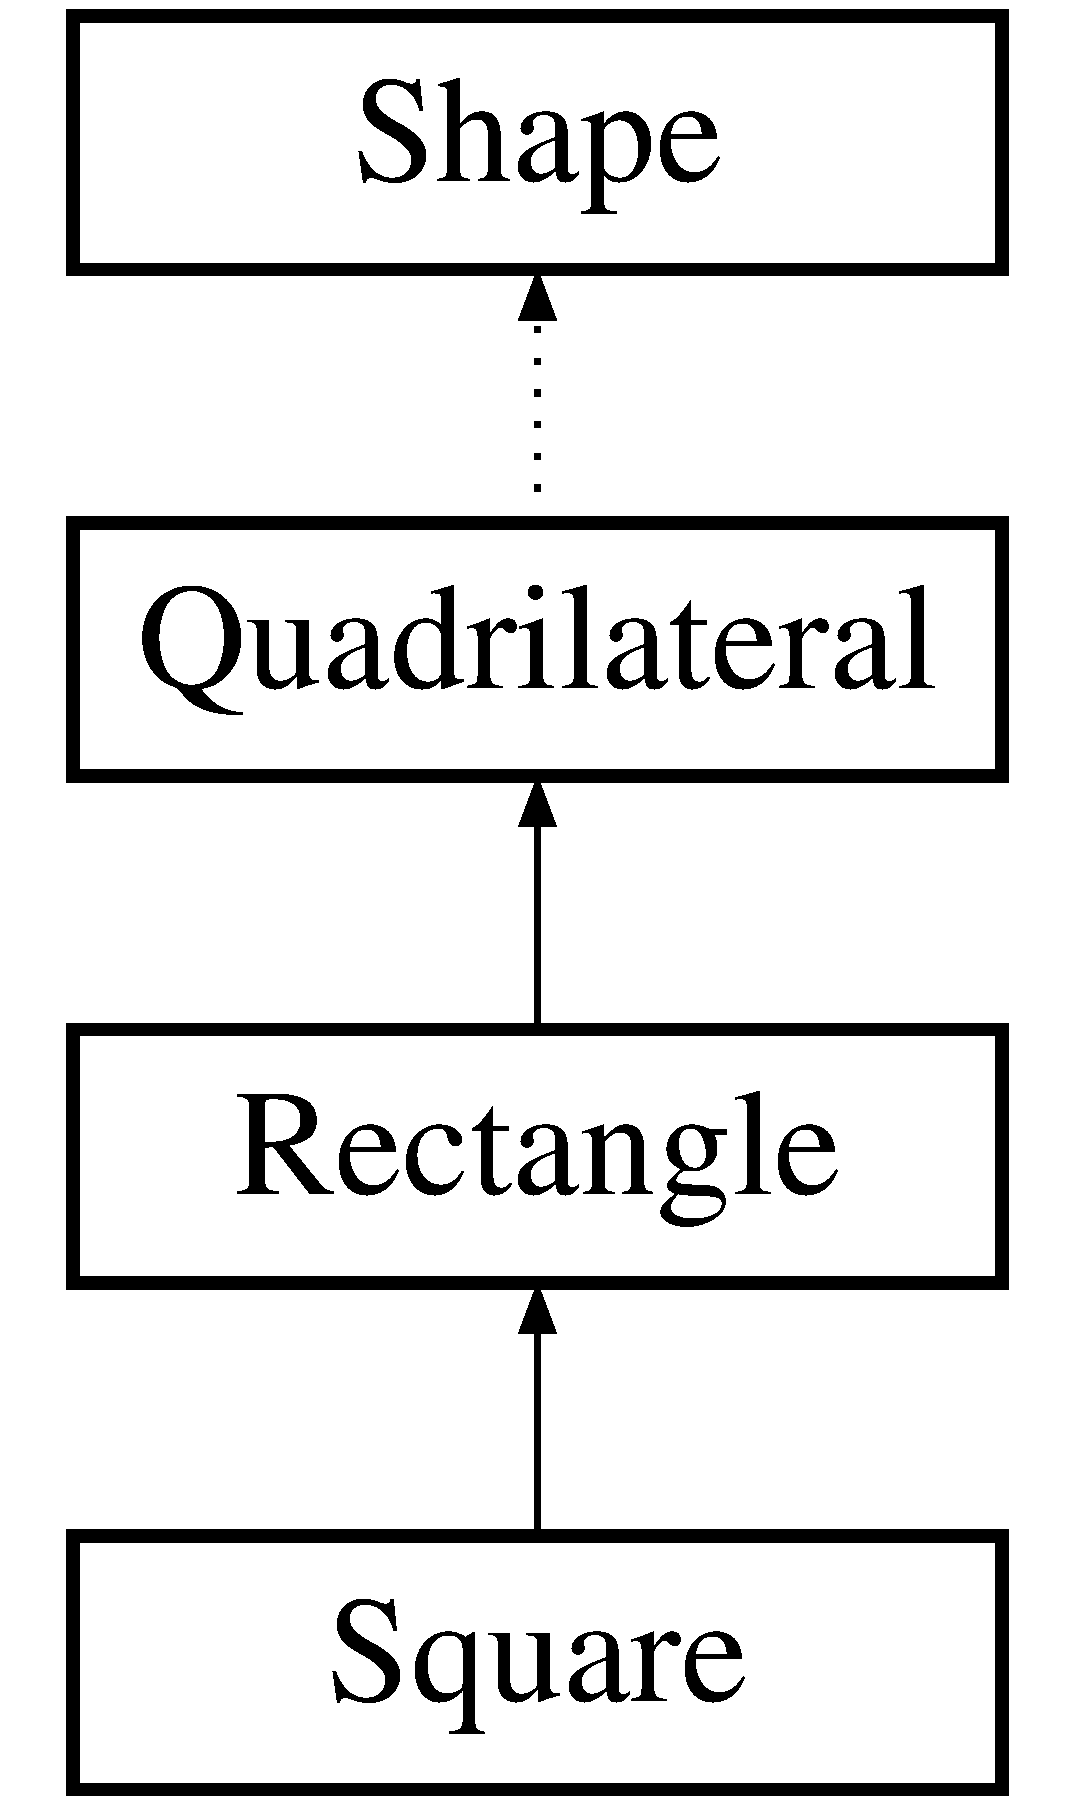
\includegraphics[height=4.000000cm]{class_quadrilateral}
\end{center}
\end{figure}
\subsection*{Public Member Functions}
\begin{DoxyCompactItemize}
\item 
\mbox{\hyperlink{class_quadrilateral_accb7341bd0b9589fc9d672822b5b3f8d}{Quadrilateral}} (\mbox{\hyperlink{class_point}{Point}} A, \mbox{\hyperlink{class_point}{Point}} B, \mbox{\hyperlink{class_point}{Point}} C, \mbox{\hyperlink{class_point}{Point}} D)
\item 
float \mbox{\hyperlink{class_quadrilateral_a254b3672c291adf79536ddb5de67f31d}{get\+Area}} ()
\item 
float \mbox{\hyperlink{class_quadrilateral_a6cbaf55455f983553b5fd8ff10c73a57}{get\+Perimeter}} ()
\end{DoxyCompactItemize}
\subsection*{Protected Attributes}
\begin{DoxyCompactItemize}
\item 
\mbox{\Hypertarget{class_quadrilateral_a65b6518cd4c2ce27c0e045a7fa99ca13}\label{class_quadrilateral_a65b6518cd4c2ce27c0e045a7fa99ca13}} 
\mbox{\hyperlink{class_point}{Point}} {\bfseries \+\_\+A}
\item 
\mbox{\Hypertarget{class_quadrilateral_afff9e71f4d844788f37851c027ed93ab}\label{class_quadrilateral_afff9e71f4d844788f37851c027ed93ab}} 
\mbox{\hyperlink{class_point}{Point}} {\bfseries \+\_\+B}
\item 
\mbox{\Hypertarget{class_quadrilateral_ade7eb0763a3bcc1323c918942896278a}\label{class_quadrilateral_ade7eb0763a3bcc1323c918942896278a}} 
\mbox{\hyperlink{class_point}{Point}} {\bfseries \+\_\+C}
\item 
\mbox{\Hypertarget{class_quadrilateral_a7fe1a2df58d2460d043dd33b75bd01de}\label{class_quadrilateral_a7fe1a2df58d2460d043dd33b75bd01de}} 
\mbox{\hyperlink{class_point}{Point}} {\bfseries \+\_\+D}
\item 
\mbox{\Hypertarget{class_quadrilateral_ae114cfa331a292abe6aa7dc8a57ffd13}\label{class_quadrilateral_ae114cfa331a292abe6aa7dc8a57ffd13}} 
bool {\bfseries \+\_\+is\+Rectangle}
\item 
\mbox{\Hypertarget{class_quadrilateral_a0790e4c00ee6410407876de1d098d020}\label{class_quadrilateral_a0790e4c00ee6410407876de1d098d020}} 
float {\bfseries \+\_\+sideA}
\item 
\mbox{\Hypertarget{class_quadrilateral_a3884b48329d7ce808eface74ac0beaa2}\label{class_quadrilateral_a3884b48329d7ce808eface74ac0beaa2}} 
float {\bfseries \+\_\+sideB}
\item 
\mbox{\Hypertarget{class_quadrilateral_aa13935280b228e3b3210d5e9cdb3f937}\label{class_quadrilateral_aa13935280b228e3b3210d5e9cdb3f937}} 
float {\bfseries \+\_\+sideC}
\item 
\mbox{\Hypertarget{class_quadrilateral_a5465e5d87329f7261552cf2b033bee38}\label{class_quadrilateral_a5465e5d87329f7261552cf2b033bee38}} 
float {\bfseries \+\_\+sideD}
\end{DoxyCompactItemize}


\subsection{Constructor \& Destructor Documentation}
\mbox{\Hypertarget{class_quadrilateral_accb7341bd0b9589fc9d672822b5b3f8d}\label{class_quadrilateral_accb7341bd0b9589fc9d672822b5b3f8d}} 
\index{Quadrilateral@{Quadrilateral}!Quadrilateral@{Quadrilateral}}
\index{Quadrilateral@{Quadrilateral}!Quadrilateral@{Quadrilateral}}
\subsubsection{\texorpdfstring{Quadrilateral()}{Quadrilateral()}}
{\footnotesize\ttfamily Quadrilateral\+::\+Quadrilateral (\begin{DoxyParamCaption}\item[{\mbox{\hyperlink{class_point}{Point}}}]{A,  }\item[{\mbox{\hyperlink{class_point}{Point}}}]{B,  }\item[{\mbox{\hyperlink{class_point}{Point}}}]{C,  }\item[{\mbox{\hyperlink{class_point}{Point}}}]{D }\end{DoxyParamCaption})}

Points must be in order 
\begin{DoxyParams}{Parameters}
{\em A} & top left corner \\
\hline
{\em B} & top right corner \\
\hline
{\em C} & bottom right corner \\
\hline
{\em D} & bottom left corner \\
\hline
\end{DoxyParams}


\subsection{Member Function Documentation}
\mbox{\Hypertarget{class_quadrilateral_a254b3672c291adf79536ddb5de67f31d}\label{class_quadrilateral_a254b3672c291adf79536ddb5de67f31d}} 
\index{Quadrilateral@{Quadrilateral}!get\+Area@{get\+Area}}
\index{get\+Area@{get\+Area}!Quadrilateral@{Quadrilateral}}
\subsubsection{\texorpdfstring{get\+Area()}{getArea()}}
{\footnotesize\ttfamily float Quadrilateral\+::get\+Area (\begin{DoxyParamCaption}{ }\end{DoxyParamCaption})\hspace{0.3cm}{\ttfamily [virtual]}}

Get shape\textquotesingle{}s area \begin{DoxyReturn}{Returns}
\mbox{\hyperlink{class_shape}{Shape}}\textquotesingle{}s area 
\end{DoxyReturn}


Reimplemented from \mbox{\hyperlink{class_shape_a90ecb4c7a5c69481145d0d53c6e010ca}{Shape}}.

\mbox{\Hypertarget{class_quadrilateral_a6cbaf55455f983553b5fd8ff10c73a57}\label{class_quadrilateral_a6cbaf55455f983553b5fd8ff10c73a57}} 
\index{Quadrilateral@{Quadrilateral}!get\+Perimeter@{get\+Perimeter}}
\index{get\+Perimeter@{get\+Perimeter}!Quadrilateral@{Quadrilateral}}
\subsubsection{\texorpdfstring{get\+Perimeter()}{getPerimeter()}}
{\footnotesize\ttfamily float Quadrilateral\+::get\+Perimeter (\begin{DoxyParamCaption}{ }\end{DoxyParamCaption})\hspace{0.3cm}{\ttfamily [virtual]}}

Get shape\textquotesingle{}s perimeter \begin{DoxyReturn}{Returns}
\mbox{\hyperlink{class_shape}{Shape}}\textquotesingle{}s perimeter 
\end{DoxyReturn}


Reimplemented from \mbox{\hyperlink{class_shape_a3bf746915187cd97c88b77238093b950}{Shape}}.



The documentation for this class was generated from the following files\+:\begin{DoxyCompactItemize}
\item 
Quadrilateral.\+h\item 
Quadrilateral.\+cpp\end{DoxyCompactItemize}

\hypertarget{class_rectangle}{}\section{Rectangle Class Reference}
\label{class_rectangle}\index{Rectangle@{Rectangle}}
Inheritance diagram for Rectangle\+:\begin{figure}[H]
\begin{center}
\leavevmode
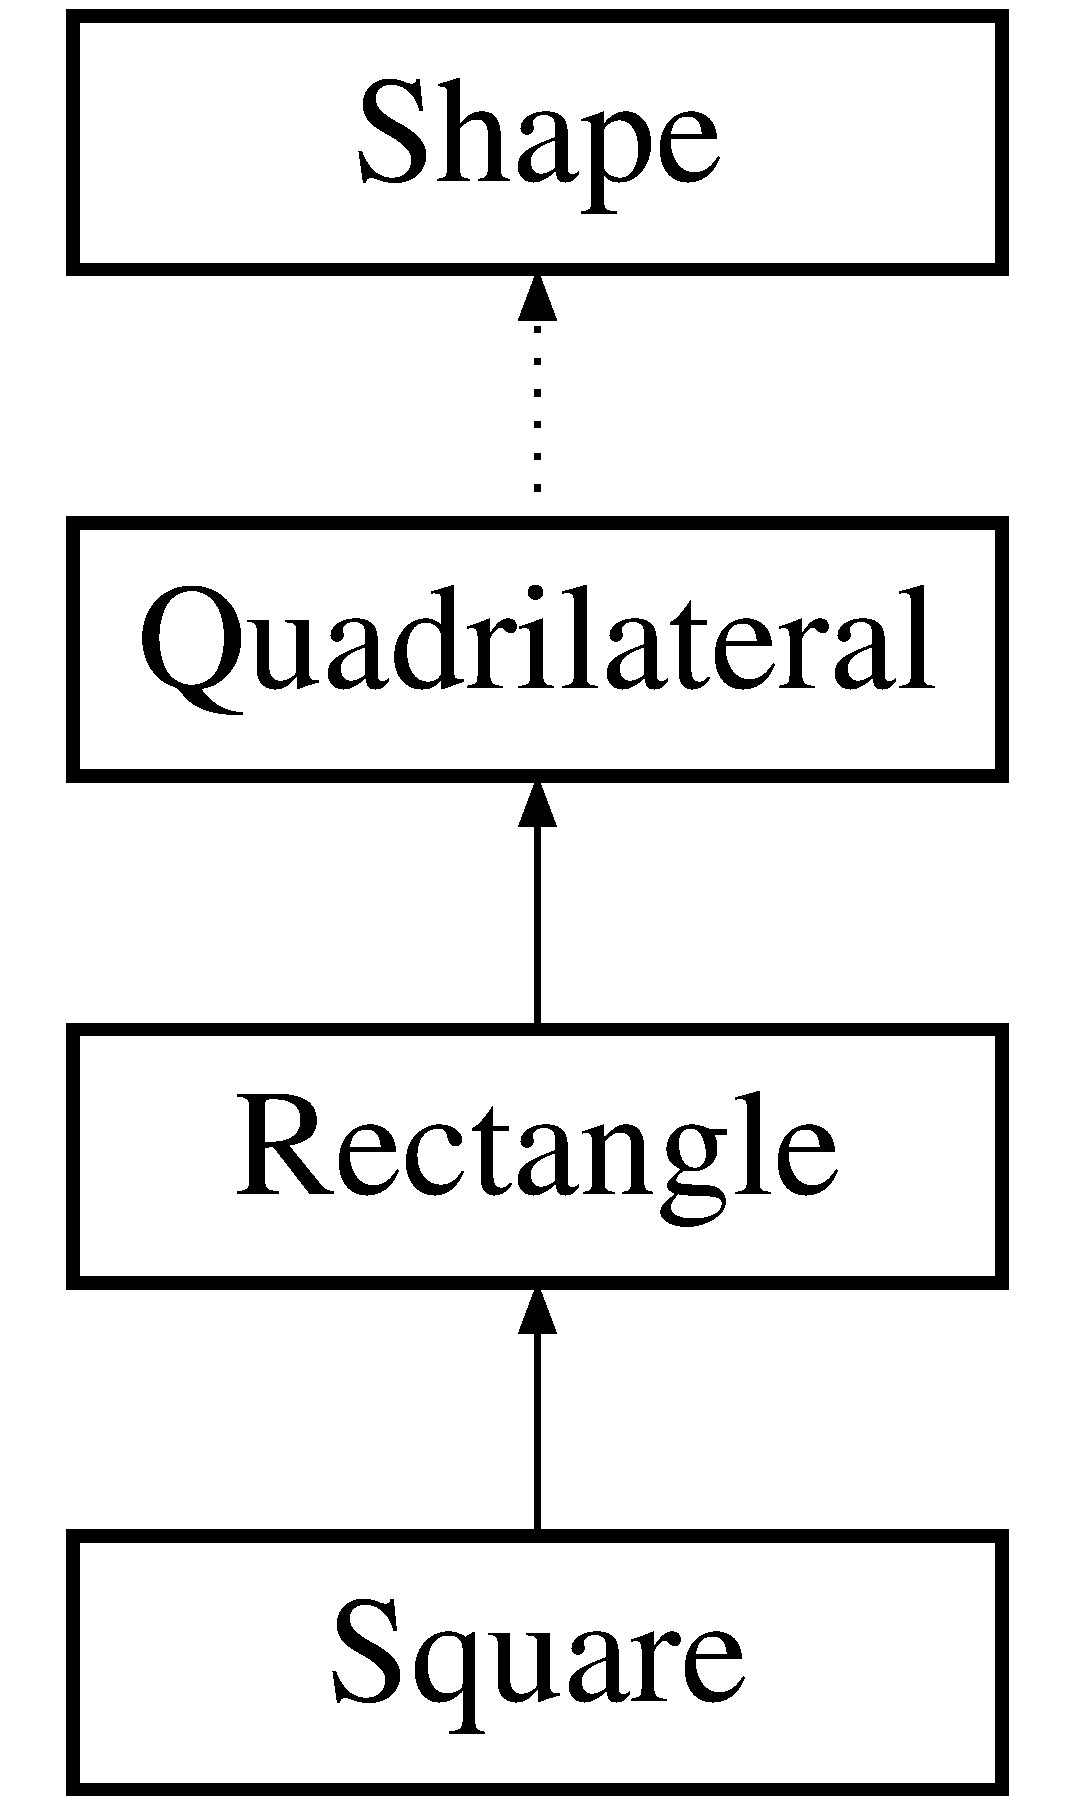
\includegraphics[height=4.000000cm]{class_rectangle}
\end{center}
\end{figure}
\subsection*{Public Member Functions}
\begin{DoxyCompactItemize}
\item 
\mbox{\Hypertarget{class_rectangle_a7c887b9c998a47ca2e1c93c9c4a3a451}\label{class_rectangle_a7c887b9c998a47ca2e1c93c9c4a3a451}} 
{\bfseries Rectangle} (\mbox{\hyperlink{class_point}{Point}} A, \mbox{\hyperlink{class_point}{Point}} B, \mbox{\hyperlink{class_point}{Point}} C, \mbox{\hyperlink{class_point}{Point}} D)
\item 
\mbox{\Hypertarget{class_rectangle_a01405cb4bc1cef7c60e16f991b12269b}\label{class_rectangle_a01405cb4bc1cef7c60e16f991b12269b}} 
bool {\bfseries is\+Rectangle} ()
\end{DoxyCompactItemize}
\subsection*{Additional Inherited Members}


The documentation for this class was generated from the following files\+:\begin{DoxyCompactItemize}
\item 
Rectangle.\+h\item 
Rectangle.\+cpp\end{DoxyCompactItemize}

\hypertarget{class_right_triangle}{}\section{Right\+Triangle Class Reference}
\label{class_right_triangle}\index{Right\+Triangle@{Right\+Triangle}}
Inheritance diagram for Right\+Triangle\+:\begin{figure}[H]
\begin{center}
\leavevmode
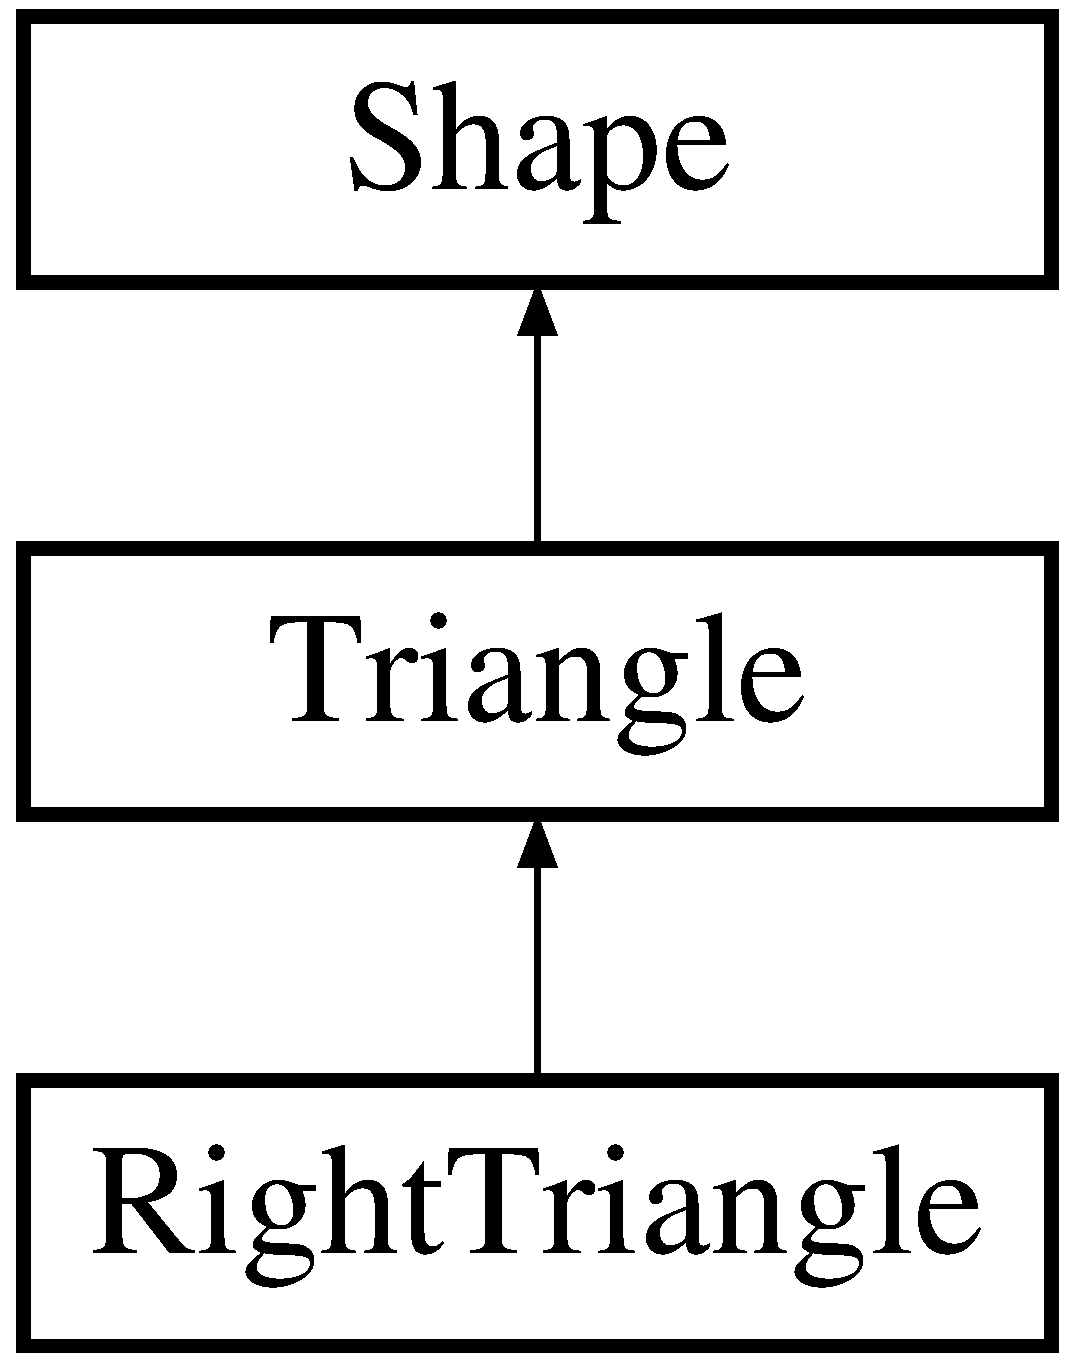
\includegraphics[height=3.000000cm]{class_right_triangle}
\end{center}
\end{figure}
\subsection*{Public Member Functions}
\begin{DoxyCompactItemize}
\item 
\mbox{\Hypertarget{class_right_triangle_a532534df65aeabb7af675f87086db6bc}\label{class_right_triangle_a532534df65aeabb7af675f87086db6bc}} 
{\bfseries Right\+Triangle} (\mbox{\hyperlink{class_point}{Point}} A, \mbox{\hyperlink{class_point}{Point}} B, \mbox{\hyperlink{class_point}{Point}} C)
\item 
bool \mbox{\hyperlink{class_right_triangle_a5dc1d7509c3909221b1902f6a6ebc2c4}{is\+Right\+Triangle}} ()
\end{DoxyCompactItemize}
\subsection*{Additional Inherited Members}


\subsection{Member Function Documentation}
\mbox{\Hypertarget{class_right_triangle_a5dc1d7509c3909221b1902f6a6ebc2c4}\label{class_right_triangle_a5dc1d7509c3909221b1902f6a6ebc2c4}} 
\index{Right\+Triangle@{Right\+Triangle}!is\+Right\+Triangle@{is\+Right\+Triangle}}
\index{is\+Right\+Triangle@{is\+Right\+Triangle}!Right\+Triangle@{Right\+Triangle}}
\subsubsection{\texorpdfstring{is\+Right\+Triangle()}{isRightTriangle()}}
{\footnotesize\ttfamily bool Right\+Triangle\+::is\+Right\+Triangle (\begin{DoxyParamCaption}{ }\end{DoxyParamCaption})}

Checking if the triangle formed by the submitted points is a right triangle. Uses Pythagoras\textquotesingle{} theorem. \begin{DoxyReturn}{Returns}
True if triangle is right 
\end{DoxyReturn}


The documentation for this class was generated from the following files\+:\begin{DoxyCompactItemize}
\item 
Right\+Triangle.\+h\item 
Right\+Triangle.\+cpp\end{DoxyCompactItemize}

\hypertarget{class_shape}{}\section{Shape Class Reference}
\label{class_shape}\index{Shape@{Shape}}
Inheritance diagram for Shape\+:\begin{figure}[H]
\begin{center}
\leavevmode
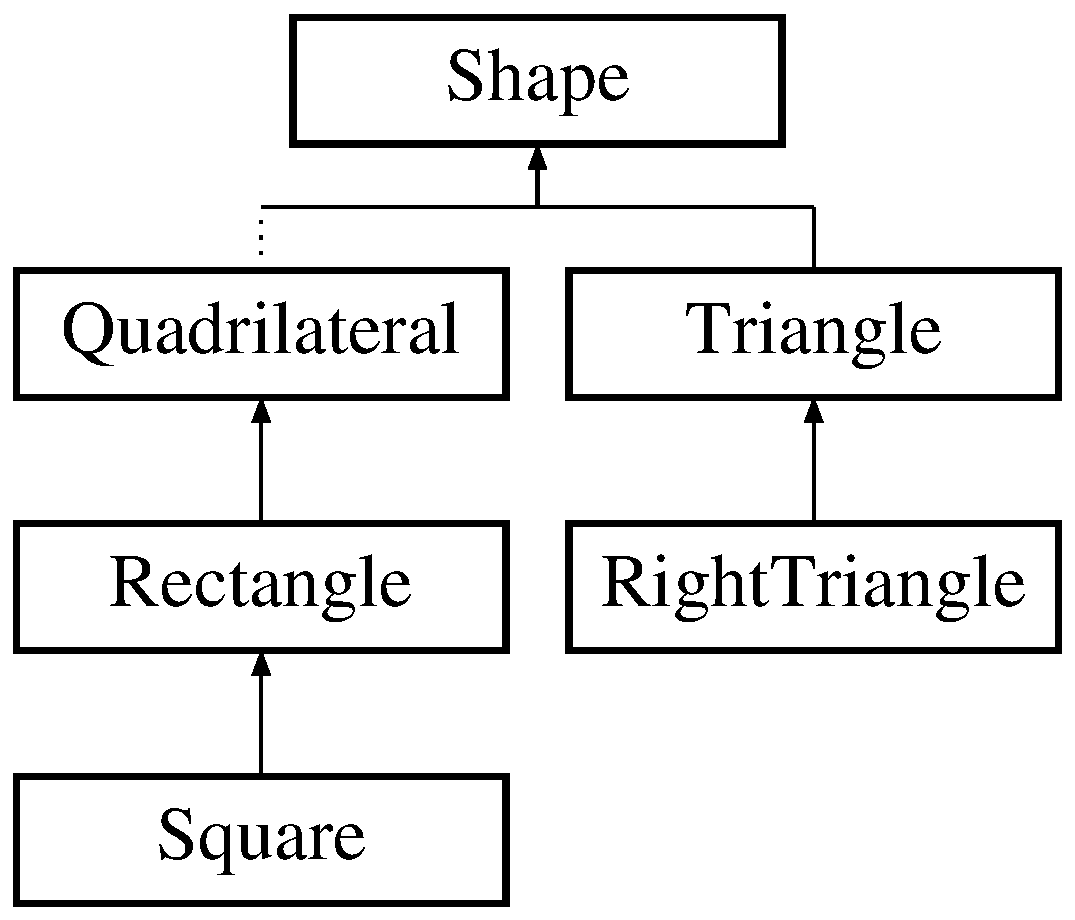
\includegraphics[height=4.000000cm]{class_shape}
\end{center}
\end{figure}
\subsection*{Public Member Functions}
\begin{DoxyCompactItemize}
\item 
virtual float \mbox{\hyperlink{class_shape_a90ecb4c7a5c69481145d0d53c6e010ca}{get\+Area}} ()
\item 
virtual float \mbox{\hyperlink{class_shape_a3bf746915187cd97c88b77238093b950}{get\+Perimeter}} ()
\end{DoxyCompactItemize}


\subsection{Member Function Documentation}
\mbox{\Hypertarget{class_shape_a90ecb4c7a5c69481145d0d53c6e010ca}\label{class_shape_a90ecb4c7a5c69481145d0d53c6e010ca}} 
\index{Shape@{Shape}!get\+Area@{get\+Area}}
\index{get\+Area@{get\+Area}!Shape@{Shape}}
\subsubsection{\texorpdfstring{get\+Area()}{getArea()}}
{\footnotesize\ttfamily virtual float Shape\+::get\+Area (\begin{DoxyParamCaption}{ }\end{DoxyParamCaption})\hspace{0.3cm}{\ttfamily [virtual]}}

Get shape\textquotesingle{}s area \begin{DoxyReturn}{Returns}
\mbox{\hyperlink{class_shape}{Shape}}\textquotesingle{}s area 
\end{DoxyReturn}


Reimplemented in \mbox{\hyperlink{class_quadrilateral_a254b3672c291adf79536ddb5de67f31d}{Quadrilateral}}, and \mbox{\hyperlink{class_triangle_a2e0ddcfb4824ea5c6a001c230c09c66c}{Triangle}}.

\mbox{\Hypertarget{class_shape_a3bf746915187cd97c88b77238093b950}\label{class_shape_a3bf746915187cd97c88b77238093b950}} 
\index{Shape@{Shape}!get\+Perimeter@{get\+Perimeter}}
\index{get\+Perimeter@{get\+Perimeter}!Shape@{Shape}}
\subsubsection{\texorpdfstring{get\+Perimeter()}{getPerimeter()}}
{\footnotesize\ttfamily virtual float Shape\+::get\+Perimeter (\begin{DoxyParamCaption}{ }\end{DoxyParamCaption})\hspace{0.3cm}{\ttfamily [virtual]}}

Get shape\textquotesingle{}s perimeter \begin{DoxyReturn}{Returns}
\mbox{\hyperlink{class_shape}{Shape}}\textquotesingle{}s perimeter 
\end{DoxyReturn}


Reimplemented in \mbox{\hyperlink{class_quadrilateral_a6cbaf55455f983553b5fd8ff10c73a57}{Quadrilateral}}, and \mbox{\hyperlink{class_triangle_aa28529a1652a1e2d75e972a5f4250f46}{Triangle}}.



The documentation for this class was generated from the following file\+:\begin{DoxyCompactItemize}
\item 
Shape.\+h\end{DoxyCompactItemize}

\hypertarget{class_square}{}\section{Square Class Reference}
\label{class_square}\index{Square@{Square}}
Inheritance diagram for Square\+:\begin{figure}[H]
\begin{center}
\leavevmode
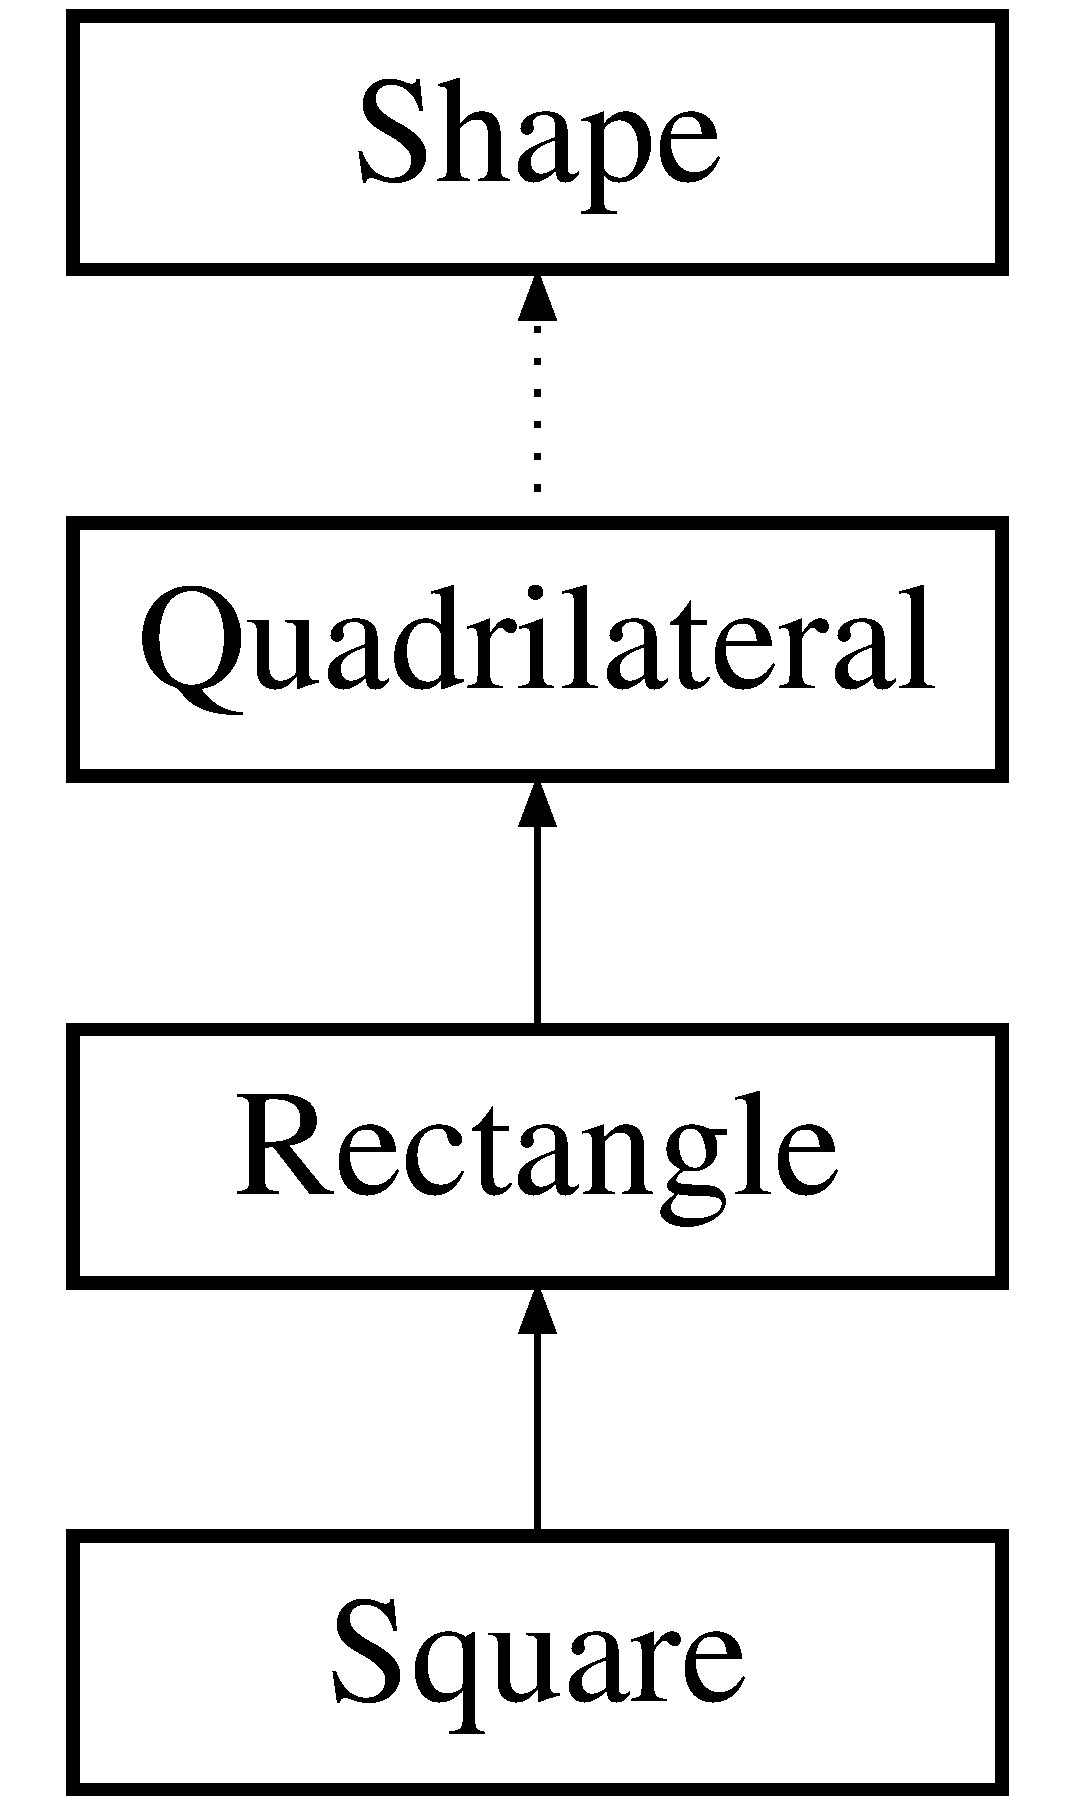
\includegraphics[height=4.000000cm]{class_square}
\end{center}
\end{figure}
\subsection*{Public Member Functions}
\begin{DoxyCompactItemize}
\item 
\mbox{\Hypertarget{class_square_a6409d9c1c814024d6450ceeeeee7865c}\label{class_square_a6409d9c1c814024d6450ceeeeee7865c}} 
{\bfseries Square} (\mbox{\hyperlink{class_point}{Point}} A, \mbox{\hyperlink{class_point}{Point}} B, \mbox{\hyperlink{class_point}{Point}} C, \mbox{\hyperlink{class_point}{Point}} D)
\item 
\mbox{\Hypertarget{class_square_a515c5d44b0238e4bad632aeefc92ebab}\label{class_square_a515c5d44b0238e4bad632aeefc92ebab}} 
bool {\bfseries is\+Square} ()
\end{DoxyCompactItemize}
\subsection*{Additional Inherited Members}


The documentation for this class was generated from the following files\+:\begin{DoxyCompactItemize}
\item 
Square.\+h\item 
Square.\+cpp\end{DoxyCompactItemize}

\hypertarget{class_triangle}{}\section{Triangle Class Reference}
\label{class_triangle}\index{Triangle@{Triangle}}
Inheritance diagram for Triangle\+:\begin{figure}[H]
\begin{center}
\leavevmode
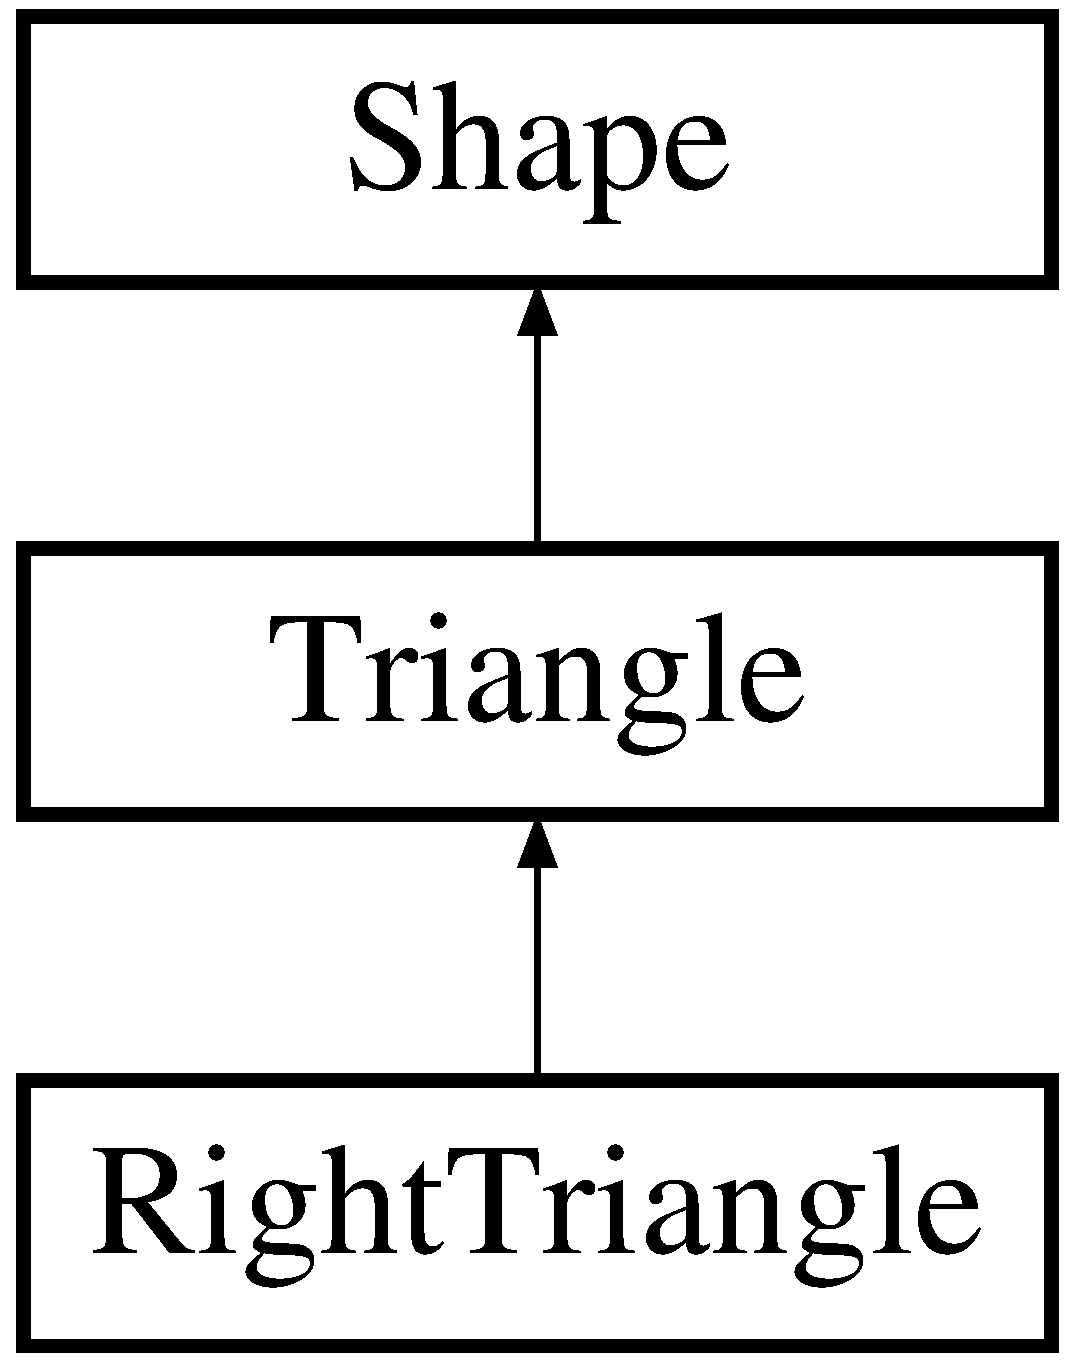
\includegraphics[height=3.000000cm]{class_triangle}
\end{center}
\end{figure}
\subsection*{Public Member Functions}
\begin{DoxyCompactItemize}
\item 
\mbox{\hyperlink{class_triangle_ae015b2eea88192163bb6e7cd93a81a35}{Triangle}} (\mbox{\hyperlink{class_point}{Point}} A, \mbox{\hyperlink{class_point}{Point}} B, \mbox{\hyperlink{class_point}{Point}} C)
\item 
float \mbox{\hyperlink{class_triangle_aa28529a1652a1e2d75e972a5f4250f46}{get\+Perimeter}} ()
\item 
float \mbox{\hyperlink{class_triangle_a2e0ddcfb4824ea5c6a001c230c09c66c}{get\+Area}} ()
\end{DoxyCompactItemize}
\subsection*{Protected Attributes}
\begin{DoxyCompactItemize}
\item 
\mbox{\Hypertarget{class_triangle_a76e5a97fcdfdabaf16c53dce3e975dd2}\label{class_triangle_a76e5a97fcdfdabaf16c53dce3e975dd2}} 
\mbox{\hyperlink{class_point}{Point}} {\bfseries \+\_\+A}
\item 
\mbox{\Hypertarget{class_triangle_a03ac8fa7ab102f088fdee42e830e821b}\label{class_triangle_a03ac8fa7ab102f088fdee42e830e821b}} 
\mbox{\hyperlink{class_point}{Point}} {\bfseries \+\_\+B}
\item 
\mbox{\Hypertarget{class_triangle_a216d555d6342ee27c36258e8c9aa6c52}\label{class_triangle_a216d555d6342ee27c36258e8c9aa6c52}} 
\mbox{\hyperlink{class_point}{Point}} {\bfseries \+\_\+C}
\item 
\mbox{\Hypertarget{class_triangle_a556ba0c1784024bb3b44f950235f1d1f}\label{class_triangle_a556ba0c1784024bb3b44f950235f1d1f}} 
float {\bfseries \+\_\+sideA}
\item 
\mbox{\Hypertarget{class_triangle_ad1f59d1c17978bf49106872fec377bed}\label{class_triangle_ad1f59d1c17978bf49106872fec377bed}} 
float {\bfseries \+\_\+sideB}
\item 
\mbox{\Hypertarget{class_triangle_a97f48eff98e5d40ea60d6b19d103dcd0}\label{class_triangle_a97f48eff98e5d40ea60d6b19d103dcd0}} 
float {\bfseries \+\_\+sideC}
\end{DoxyCompactItemize}


\subsection{Constructor \& Destructor Documentation}
\mbox{\Hypertarget{class_triangle_ae015b2eea88192163bb6e7cd93a81a35}\label{class_triangle_ae015b2eea88192163bb6e7cd93a81a35}} 
\index{Triangle@{Triangle}!Triangle@{Triangle}}
\index{Triangle@{Triangle}!Triangle@{Triangle}}
\subsubsection{\texorpdfstring{Triangle()}{Triangle()}}
{\footnotesize\ttfamily Triangle\+::\+Triangle (\begin{DoxyParamCaption}\item[{\mbox{\hyperlink{class_point}{Point}}}]{A,  }\item[{\mbox{\hyperlink{class_point}{Point}}}]{B,  }\item[{\mbox{\hyperlink{class_point}{Point}}}]{C }\end{DoxyParamCaption})}


\begin{DoxyParams}{Parameters}
{\em A} & A corner of the triangle \\
\hline
{\em B} & Another corner of the triangle \\
\hline
{\em C} & Another corner of the triangle \\
\hline
\end{DoxyParams}


\subsection{Member Function Documentation}
\mbox{\Hypertarget{class_triangle_a2e0ddcfb4824ea5c6a001c230c09c66c}\label{class_triangle_a2e0ddcfb4824ea5c6a001c230c09c66c}} 
\index{Triangle@{Triangle}!get\+Area@{get\+Area}}
\index{get\+Area@{get\+Area}!Triangle@{Triangle}}
\subsubsection{\texorpdfstring{get\+Area()}{getArea()}}
{\footnotesize\ttfamily float Triangle\+::get\+Area (\begin{DoxyParamCaption}{ }\end{DoxyParamCaption})\hspace{0.3cm}{\ttfamily [virtual]}}

Get shape\textquotesingle{}s area \begin{DoxyReturn}{Returns}
\mbox{\hyperlink{class_shape}{Shape}}\textquotesingle{}s area 
\end{DoxyReturn}


Reimplemented from \mbox{\hyperlink{class_shape_a90ecb4c7a5c69481145d0d53c6e010ca}{Shape}}.

\mbox{\Hypertarget{class_triangle_aa28529a1652a1e2d75e972a5f4250f46}\label{class_triangle_aa28529a1652a1e2d75e972a5f4250f46}} 
\index{Triangle@{Triangle}!get\+Perimeter@{get\+Perimeter}}
\index{get\+Perimeter@{get\+Perimeter}!Triangle@{Triangle}}
\subsubsection{\texorpdfstring{get\+Perimeter()}{getPerimeter()}}
{\footnotesize\ttfamily float Triangle\+::get\+Perimeter (\begin{DoxyParamCaption}{ }\end{DoxyParamCaption})\hspace{0.3cm}{\ttfamily [virtual]}}

Get shape\textquotesingle{}s perimeter \begin{DoxyReturn}{Returns}
\mbox{\hyperlink{class_shape}{Shape}}\textquotesingle{}s perimeter 
\end{DoxyReturn}


Reimplemented from \mbox{\hyperlink{class_shape_a3bf746915187cd97c88b77238093b950}{Shape}}.



The documentation for this class was generated from the following files\+:\begin{DoxyCompactItemize}
\item 
Triangle.\+h\item 
Triangle.\+cpp\end{DoxyCompactItemize}

%--- End generated contents ---

% Index
\backmatter
\newpage
\phantomsection
\clearemptydoublepage
\addcontentsline{toc}{chapter}{Index}
\printindex

\end{document}
